\ifthenelse{\equal{\Langue}{FR}}{
    \chapter{Alimentation d'un microprocesseur}
}{
    \chapter{Powering a microprocessor}
}

\ifthenelse{\equal{\Langue}{FR}}{
    On souhaite alimenter un microprocesseur STM32H4 à l'aide d'une batterie. Le cahier des charges est le suivant:
}{
    We want to power an STM32H4 microprocessor using a battery. The specifications are as follows:

}

\begin{itemize}
\ifthenelse{\equal{\Langue}{FR}}{
    \item Batterie LiPo 2S $V_{in} = 7.4\ V$
    \item Tension d'alimentation du microprocesseur: $V_{out}=3.3\ V$
    \item Ondulation de tension max en entrée du microprocesseur: $\Delta V_S = 50\ mV$
    \item Courant nominal de sortie: $I_S = 200\ mA$
    \item Ondulation de courant: 30\%
}{
    \item LiPo 2S battery $V_{in} = 7.4\ V$
    \item Microprocessor supply voltage: $V_{out}=3.3\ V$
    \item Maximum voltage ripple at the microprocessor input: $\Delta V_S = 50\ mV$
    \item Output nominal current: $I_S = 200\ mA$
    \item Current ripple: 30\%
}
\end{itemize}

\ifthenelse{\equal{\Langue}{FR}}{
    Pour cela, on souhaite utiliser le composant suivant: \textbf{LT1959} dont un extrait de la documentation est en annexe. Afin de dimensionner tous les composants, on décide d'utiliser des IAg: Claude (Sonnet 4.6), Copilot (M365 Copilot basé sur GPT-5.5 Automatique) et ChatGPT (GPT 5.5 Instant). Les réponses des IAs ont été générées en juin 2026. Voici le Prompt utilisé:
    

\textit{``Je souhaite utiliser le composant LT1959, pour alimenter un STM32H4 à l'aide d'une batterie. Voici le cahier des charges:}

\begin{itemize}
\item \textit{Batterie LiPo 2S Vin = 7.4 V}
\item \textit{Tension d'alimentation du microprocesseur: Vout = 3.3 V}
\item \textit{Ondulation de tension max en entrée du microprocesseur: $\Delta$ VS = 50 mV}
\item \textit{Courant nominal de sortie: IS = 200 mA}
\item \textit{Ondulation de courant: 30\%}
\end{itemize}   
\textit{Dans un fichier word, détaille moi les calculs pour le dimensionnement des composants passifs. Ajoute une image du schéma électrique. Ajoute une autre image avec la forme du courant dans l'inductance, de la tension sur la broche SW et de la tension de sortie''.}
}{
    To achieve this, we want to use the following component: \textbf{LT1959}, an excerpt of the documentation is attached. To size all the components, we decided to use IAs: Claude (Sonnet 4.6), Copilot (M365 Copilot based on GPT-5.5 Automatic) and ChatGPT (GPT 5.5 Instant). The AI responses were generated in June 2026 in French and then translated in English (the original Prompt and responses are in the French version of this Tutorial). Here is the translation in English of the prompt used:

\textit{``I want to use the LT1959 component to power an STM32H4 using a battery. Here are the specifications:}

\begin{itemize}
\item \textit{LiPo 2S battery Vin = 7.4 V}
\item \textit{Microprocessor supply voltage: Vout = 3.3 V}
\item \textit{Maximum voltage ripple at the microprocessor input: $\Delta$ VS = 50 mV}
\item \textit{Output nominal current: IS = 200 mA}
\item \textit{Current ripple: 30\%}
\end{itemize}   
\textit{In a Word file, detail the calculations for the sizing of passive components. Add an image of the electrical schematic. Add another image with the waveform of the current in the inductance, the voltage on the SW pin, and the output voltage''.}
}

\vspace{0.5cm}
\ifthenelse{\equal{\Langue}{FR}}{
A partir des réponses des IAs et de vos connaissances:
}
{
With the AI responses and your knowledge:
}

\begin{enumerate}
\ifthenelse{\equal{\Langue}{FR}}{
\item Représenter le schéma électrique du convertisseur Buck
\item Donner les formes d'ondes de la tension sur la broche SW, du courant dans l'inductance et de la tension de sortie (en supposant que l'ondulation de tension vient principalement de l'ESR du condensateur)
\item Dimensionner les composants passifs du convertisseur Buck
}{
\item Draw the electrical schematic of the Buck converter
\item Give the waveforms of the voltage on the SW pin, the current in the inductor, and the output voltage (assuming that the voltage ripple comes mainly from the ESR of the capacitor)
\item Size the passive components of the Buck converter
}



\end{enumerate}


\newpage
\ifthenelse{\equal{\Langue}{FR}}{
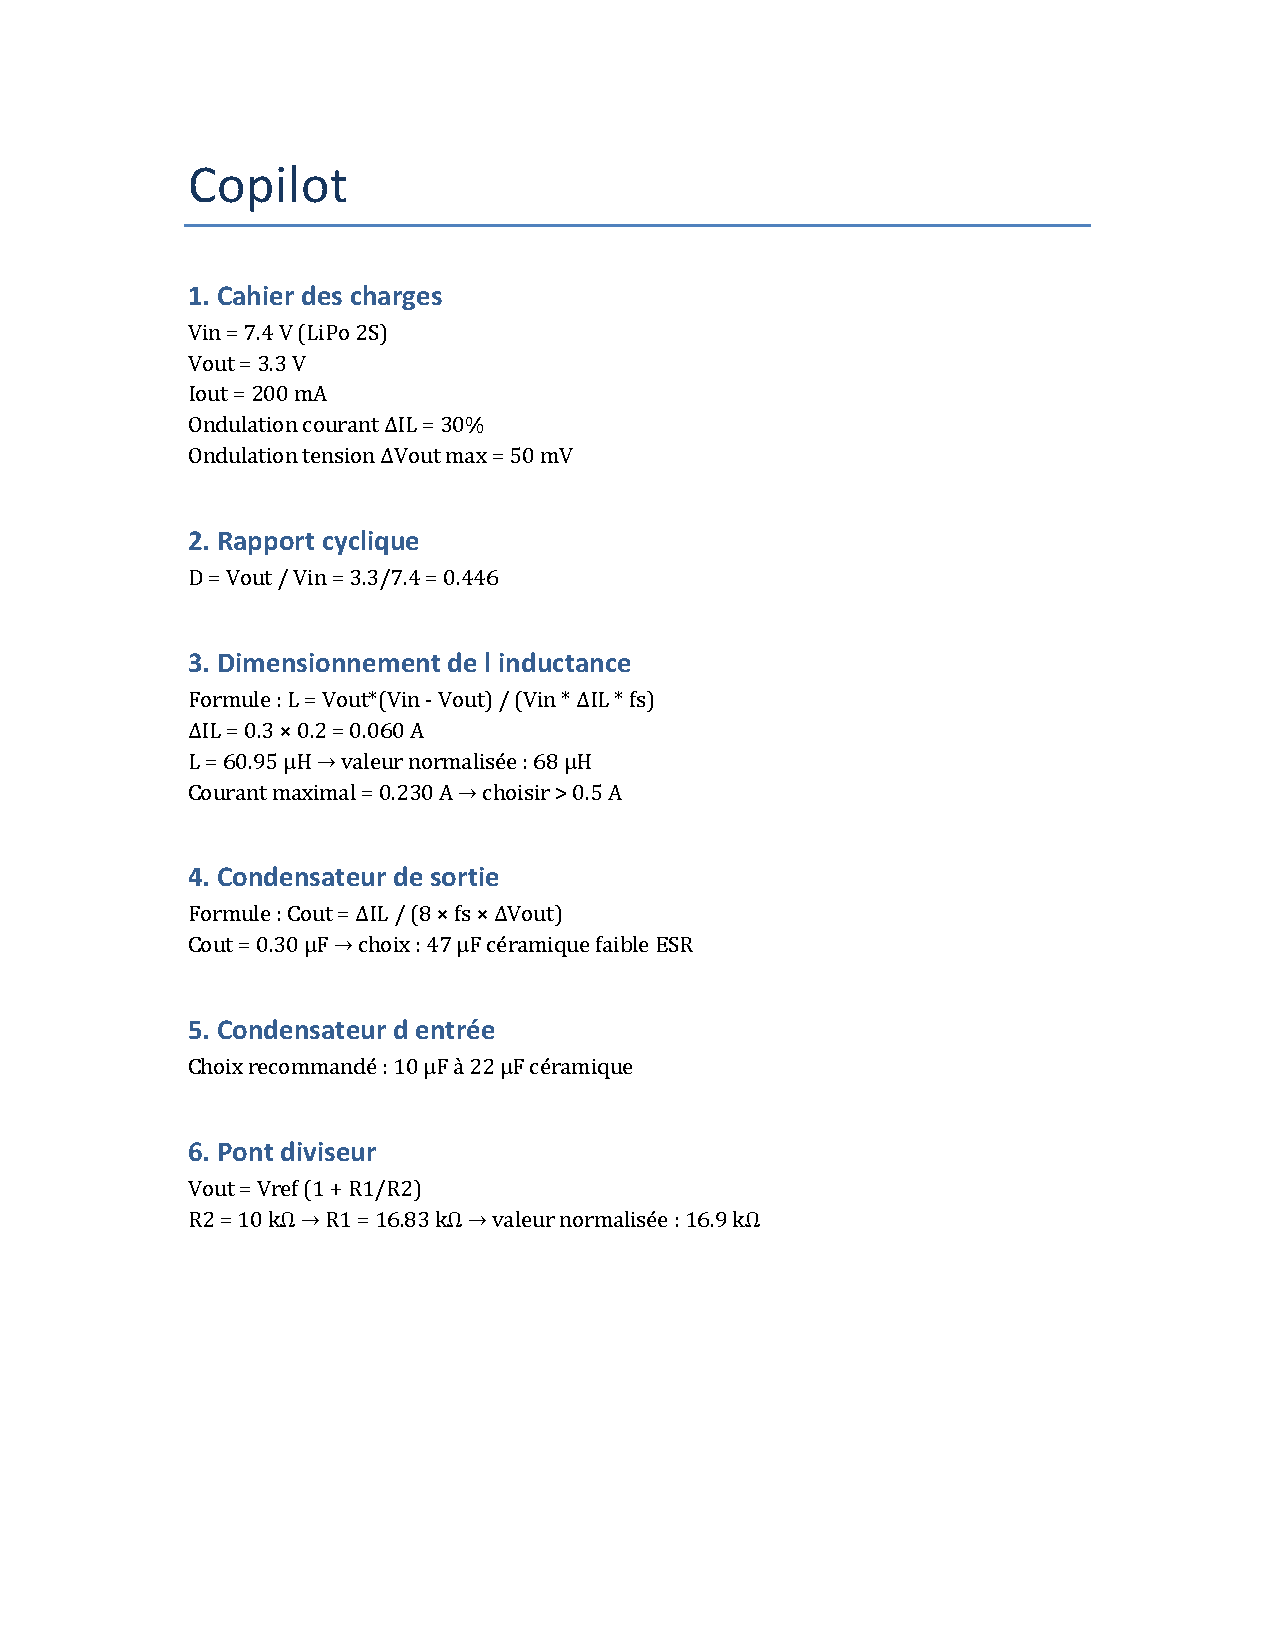
\includepdf[pages=-]{TD_Buck_IA/Réponses_IA/Reponse_Copilot_FR.pdf}
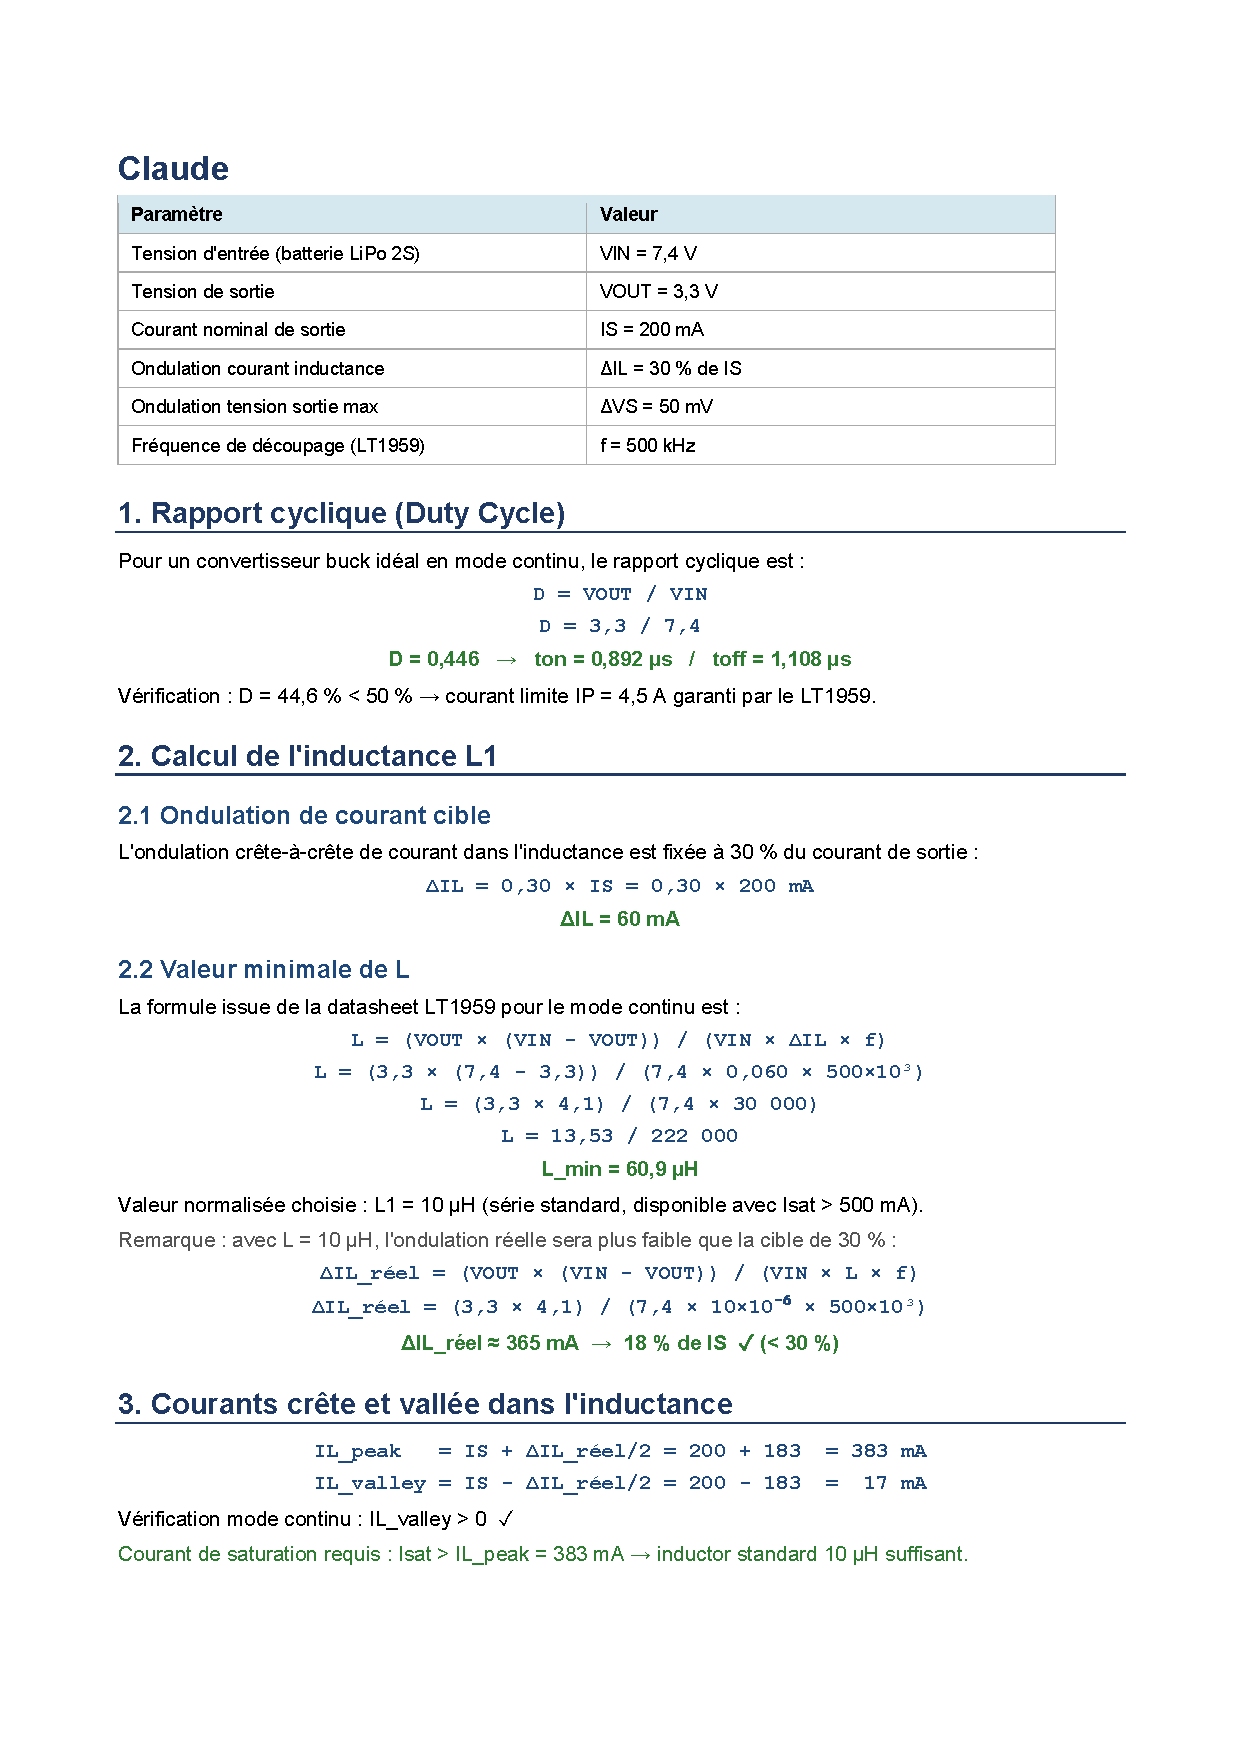
\includepdf[pages=-]{TD_Buck_IA/Réponses_IA/Reponse_Claude_FR.pdf}
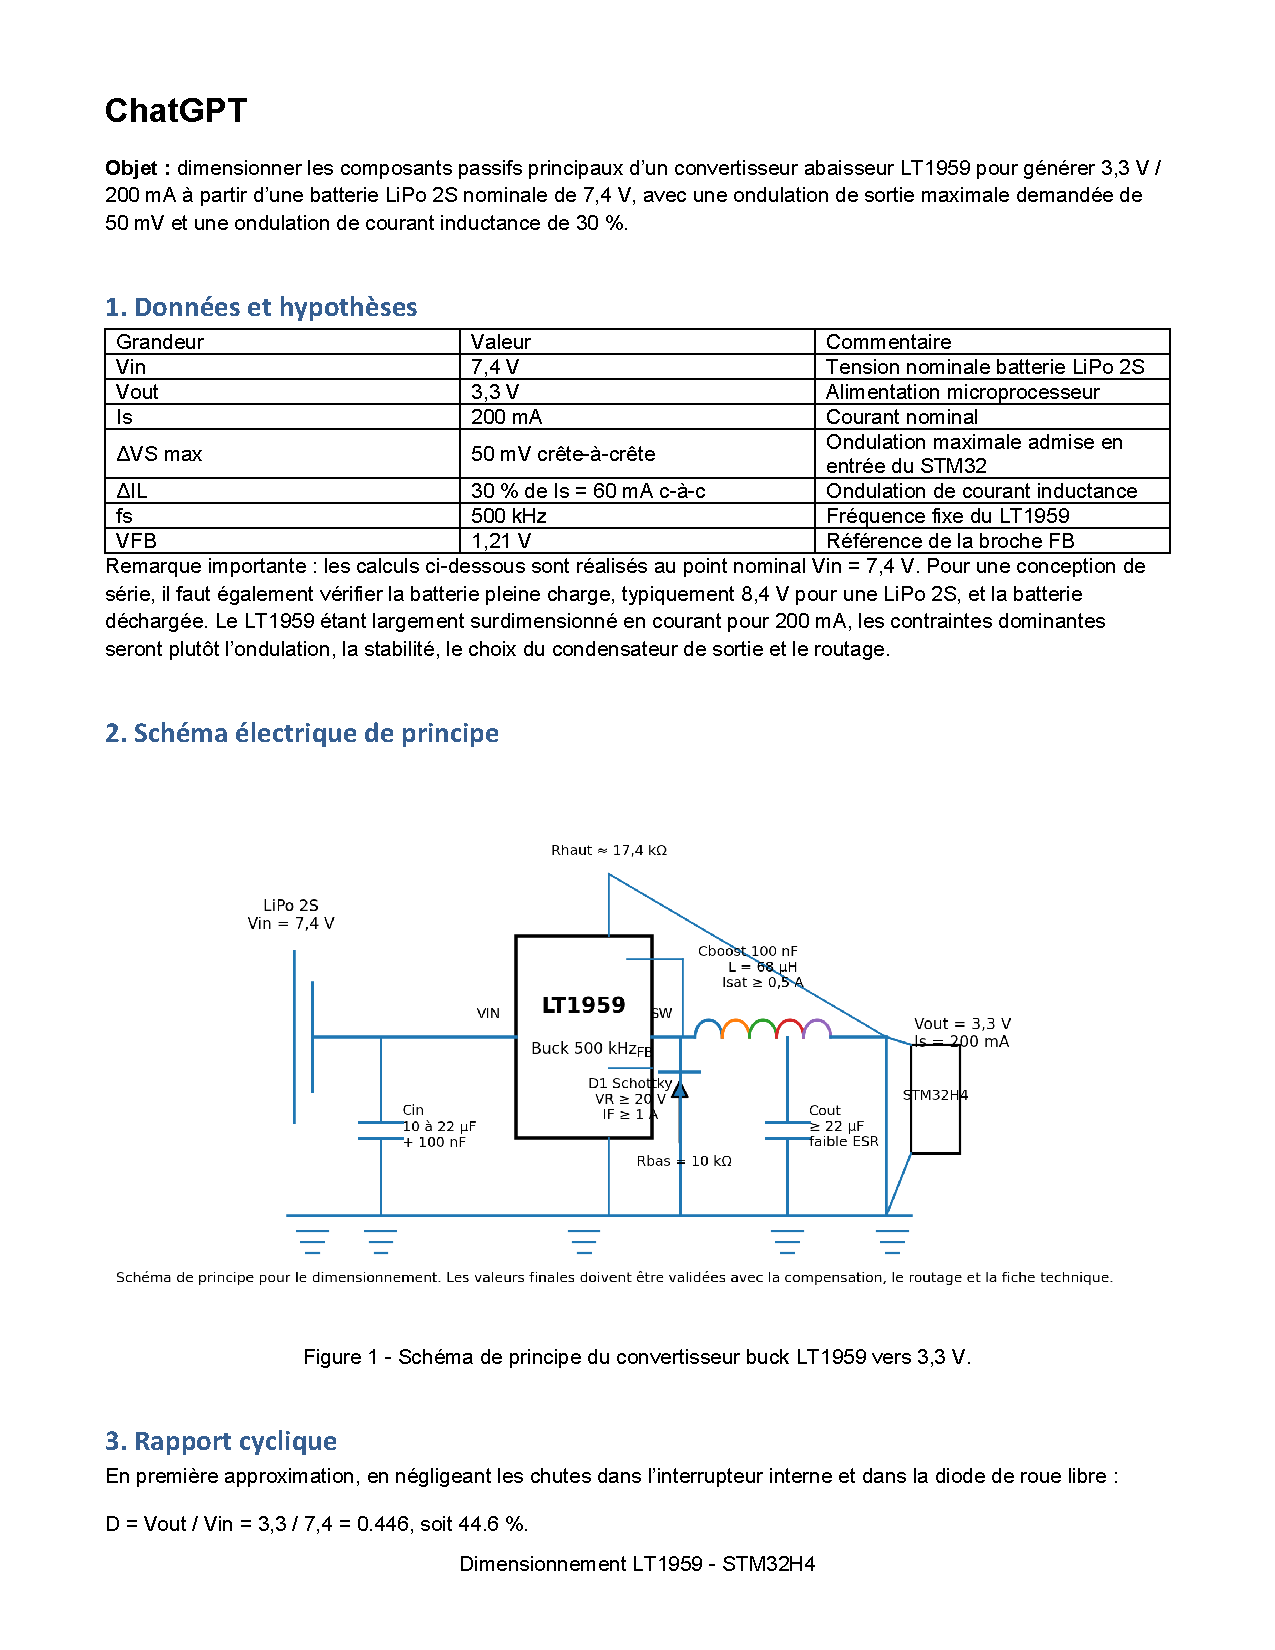
\includepdf[pages=-]{TD_Buck_IA/Réponses_IA/Reponse_ChatGPT_FR.pdf}
}{
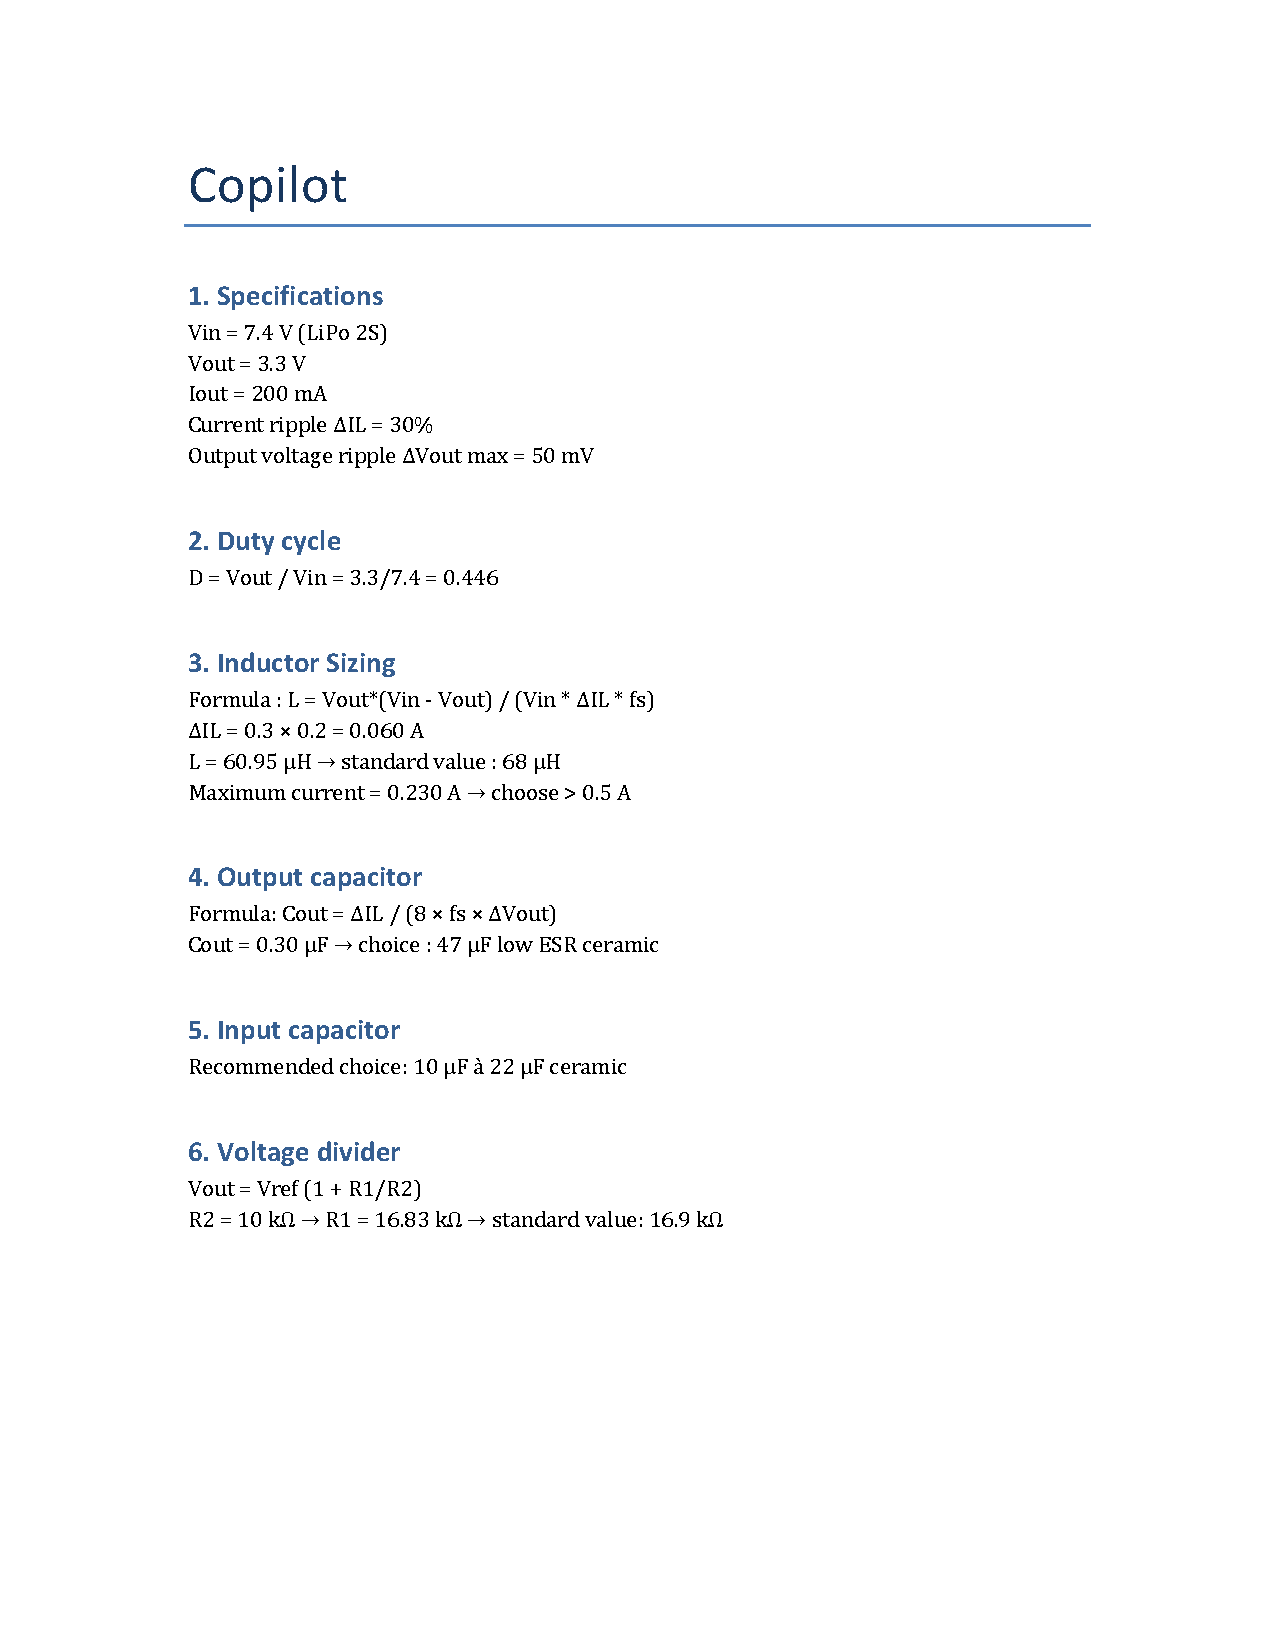
\includepdf[pages=-]{TD_Buck_IA/Réponses_IA/Reponse_Copilot_EN.pdf}
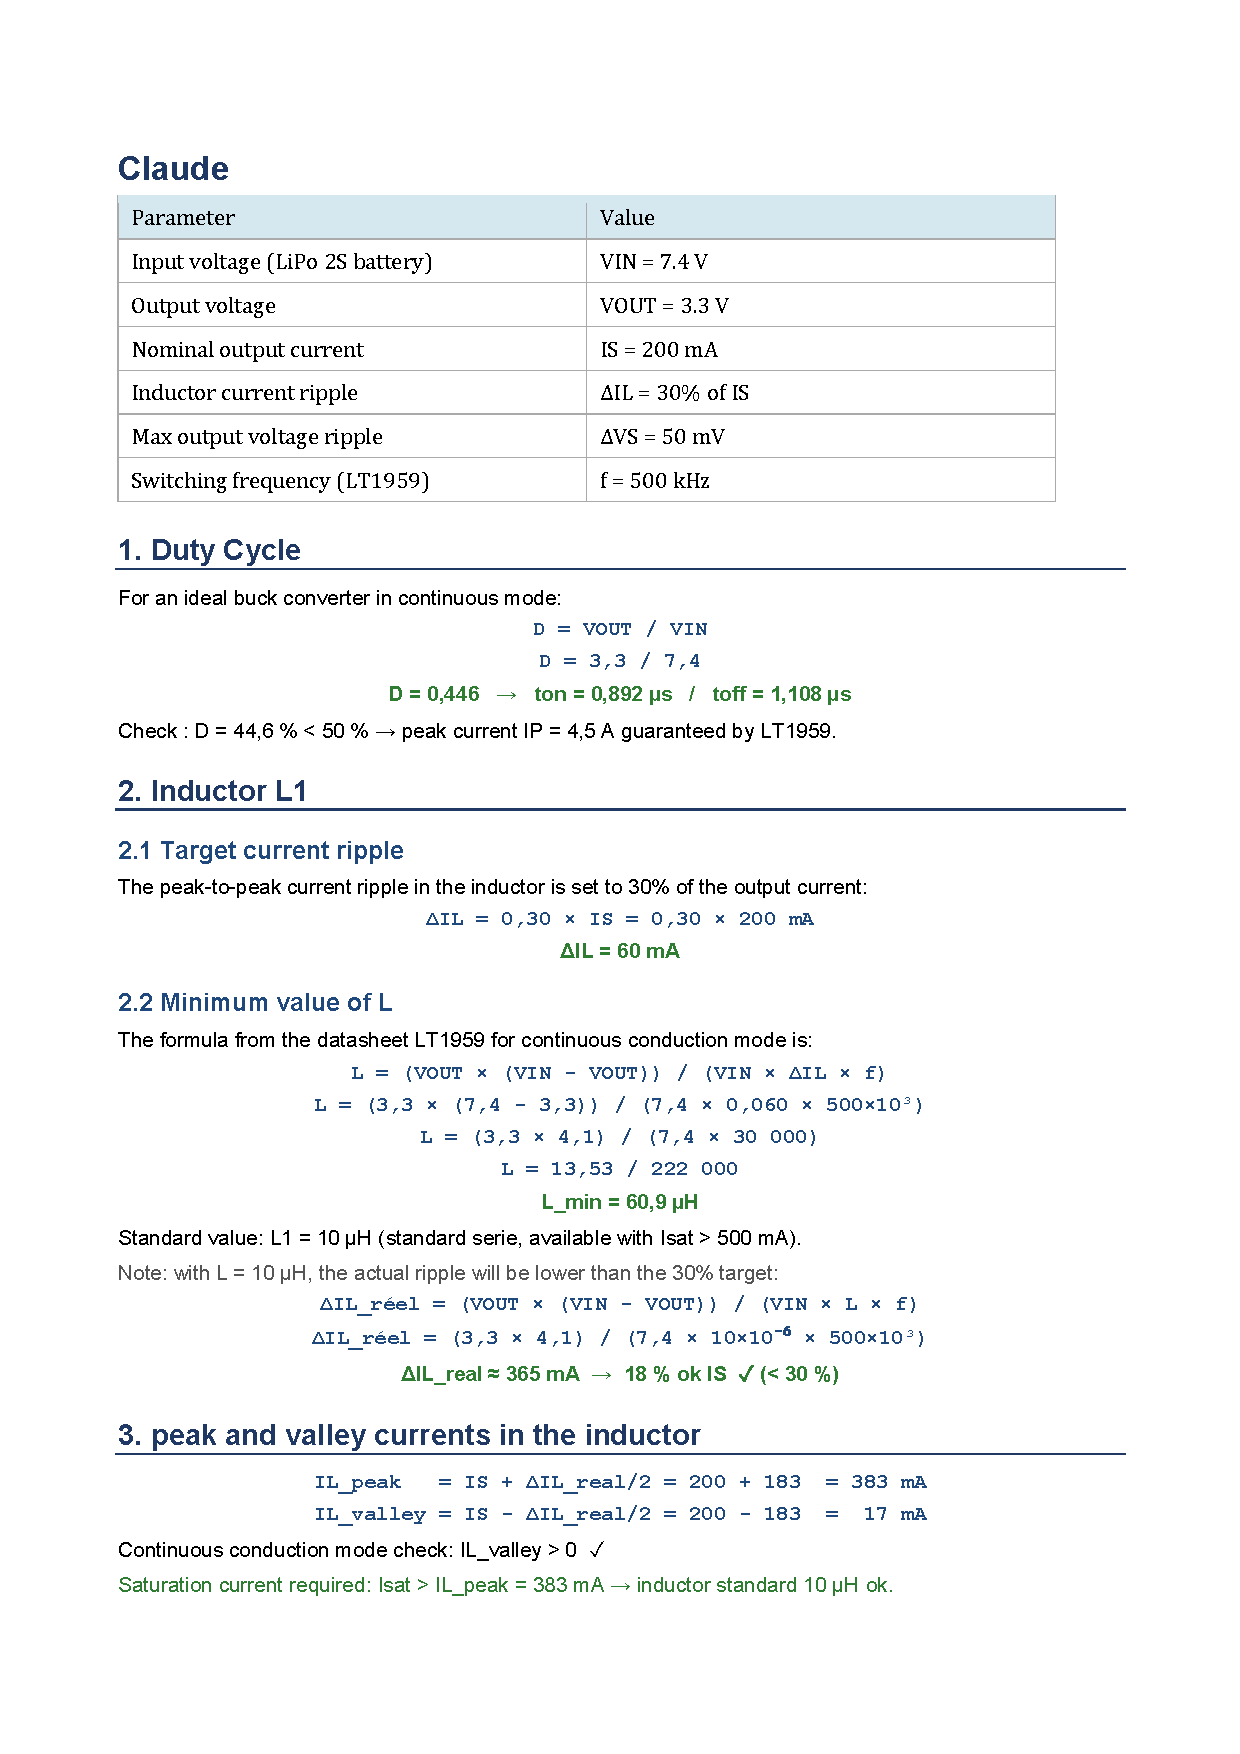
\includepdf[pages=-]{TD_Buck_IA/Réponses_IA/Reponse_Claude_EN.pdf}
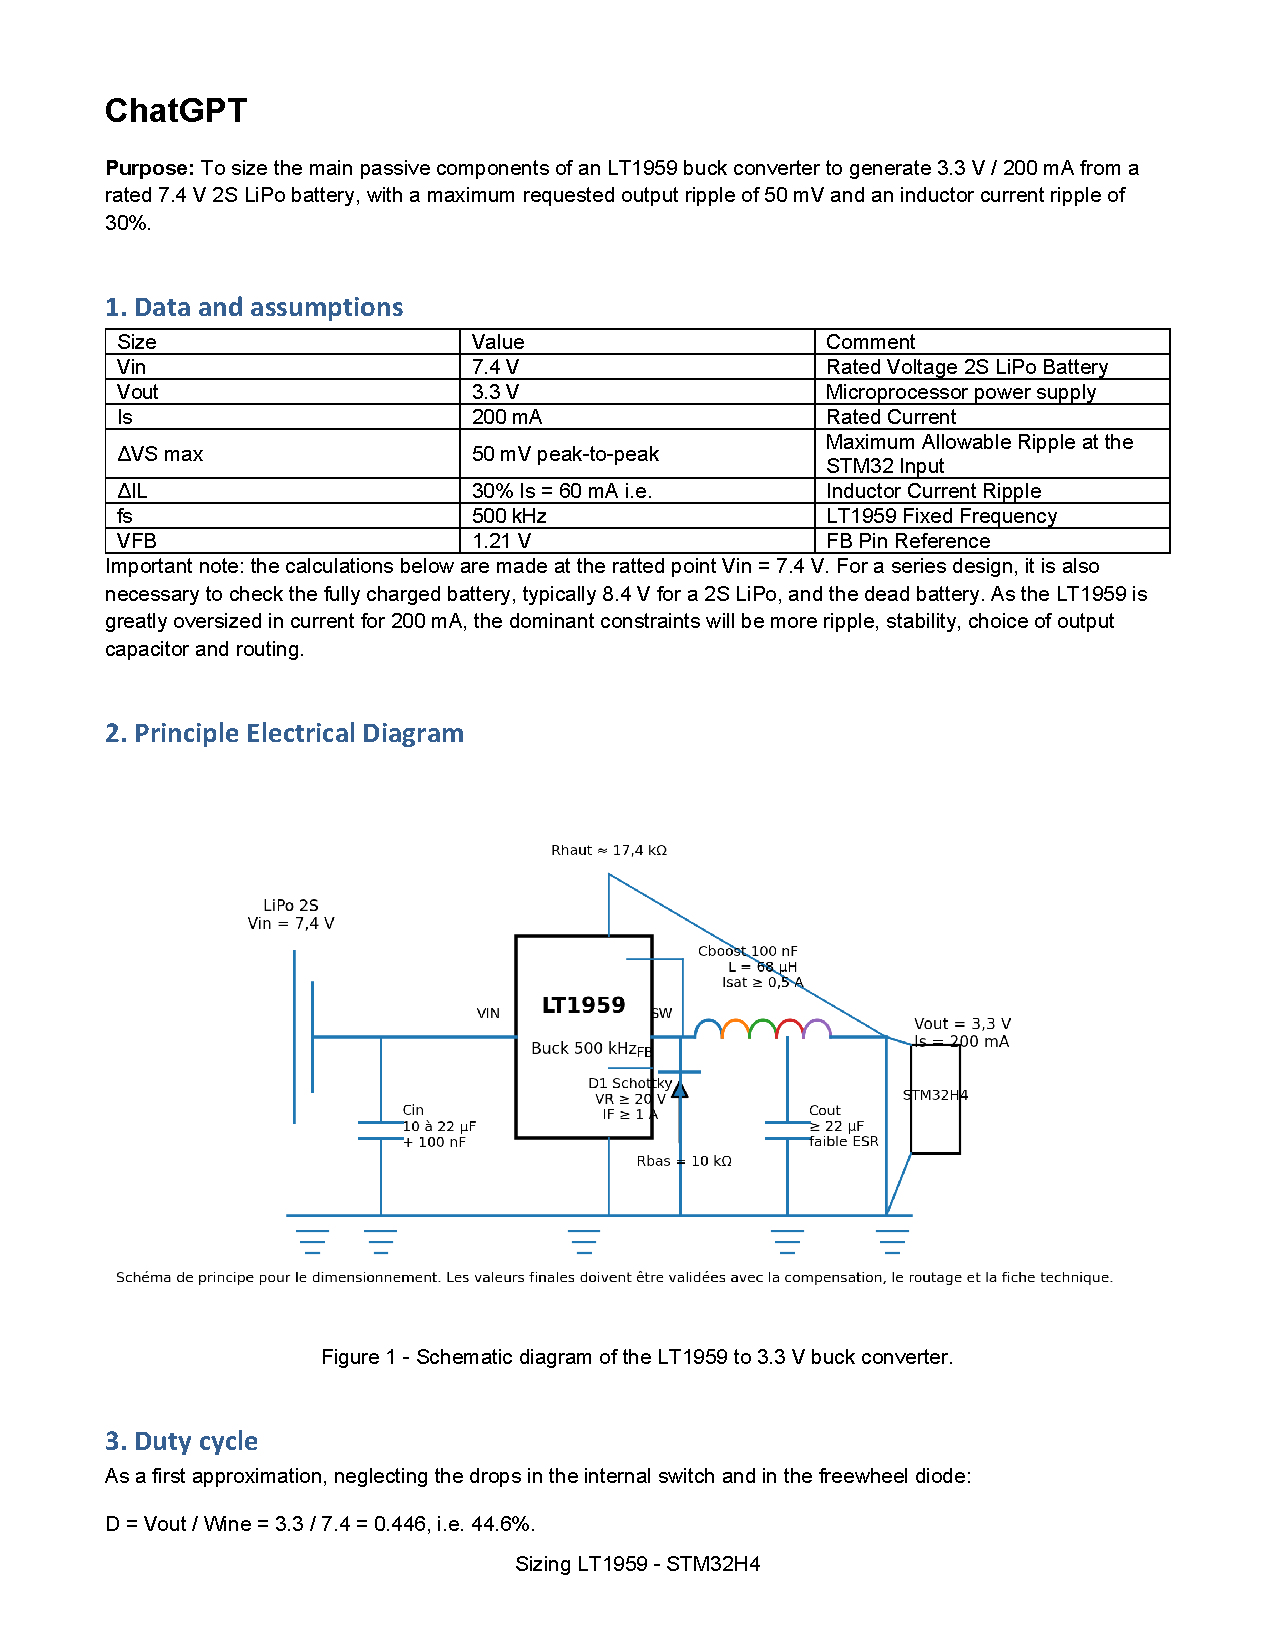
\includepdf[pages=-]{TD_Buck_IA/Réponses_IA/Reponse_ChatGPT_EN.pdf}
}

\newpage
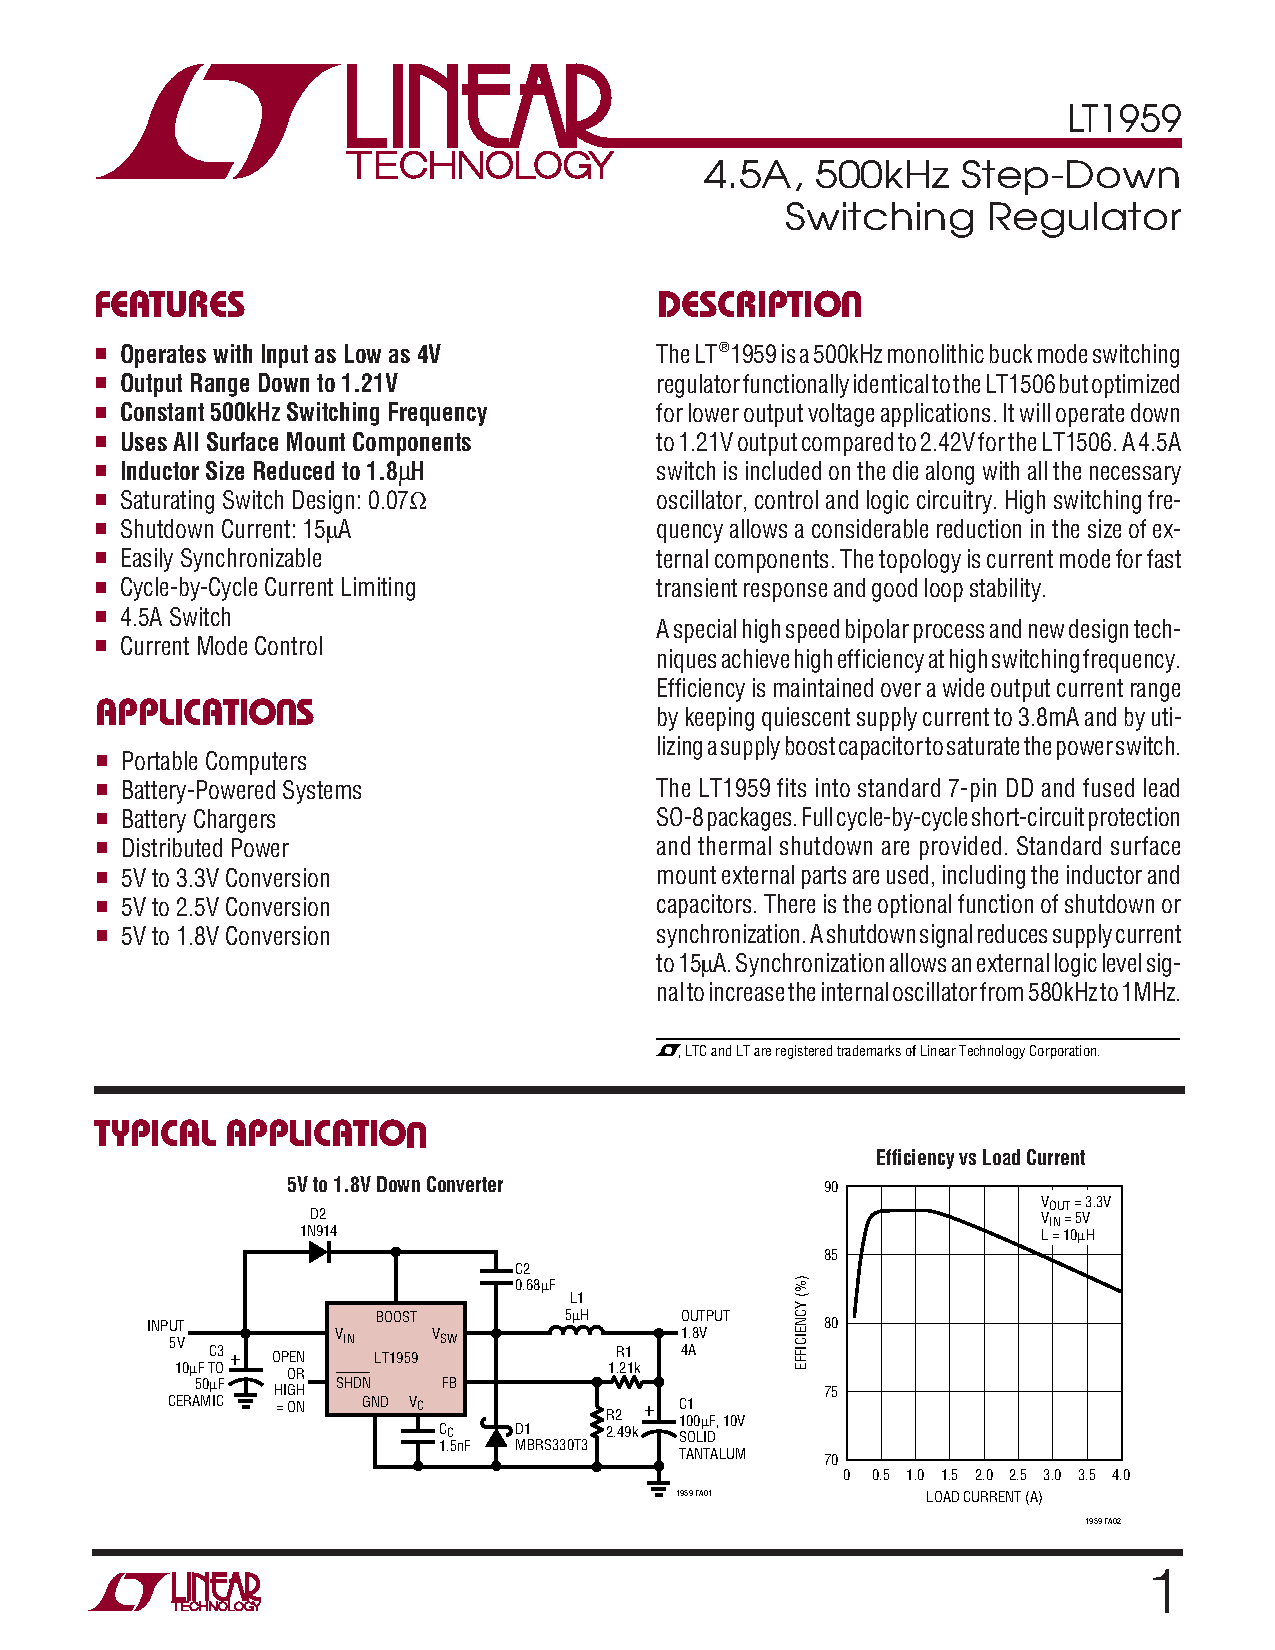
\includepdf[pages={1-13}]{TD_Buck/fig/LT1959.pdf}
%\includepdf[pages={6,7}]{TD_Buck/fig/LT1959.pdf}